\chapter{The COMET Experiment}\label{chapter2}

% \begin{markdown}
% ---

% - Description of the COMET experiment's goal, design with nice illustrations
%     + *Reference next chapter for geometry renderings*
%     + Signal and background:
%         + mu-e conv signal description
%         + **List of background sources**
% + CyDet:
%     + For simulation section, need to explain how CDC and CTH work, and how
%       combined they enable mu--e conv measurement
%     - Detailed description of the CDC, which is crucial for the GAN section.
%      - Stereo angles
% + Phase alpha?

% - References: TDR, SINDRUM II, 

% ---

% + Requirements: high sensitivity to signal, efficient rejection of backgrounds
%  + -> Need intense muon beam, pulsed, and detector design must avoid
%    backgrounds
% + TIMING of signal (muon lifetime)
% + Proton beam energy: why 8 Gev -> antiproton production
% + Intensity: beam current, beam power, POTs per second
% + Send backward-going secondaries to detector, discard the main part of
%   secondaries (forward-going)
% + Curved solenoid + dipole field (by tilting coils, see Krikler)
% + Stopping target -> why Al
% + Bunch structure, extinction
% + Phase-I detectors: StrECAL and CyDet

% ---
% \end{markdown}

% Description and goals
COMET (COherent Muon-to-Electron Transition) is a future muon-beam experiment
designed to search for the muon-to-electron conversion
process~\cite{the_comet_collaboration_comet_2020}. It is currently under
construction at the Japan Proton Accelerator Research Complex (J-PARC) facility
in Tokai, Japan. The goal of COMET is to be \numprint{10000} times more
sensitive to $\mu$--$e$ conversion than the current world-leading limit set by
the SINDRUM II experiment~\cite{Bertl:2006up}. 

% Requirements
In order to reach these goals, the COMET experiment is designed with strict
requirements defined to make the conversion signal as clear as possible, while
efficiently rejecting background events. The essential requirements that define
the COMET experiment are:
\begin{itemize}
    \item An intense muon source to probe the rare conversion process;
    \item A pulsed beam such that timing information can be used to reject backgrounds;
    \item Strict selection of charge and momentum of beam particles prior to
    reaching the detector;
    \item A tracking detector to search for the \SI{104.97}{\MeV} conversion signature.
\end{itemize}
These requirements and the design choices that were made to address them are
described in more detail in the rest of this chapter.
% Later, go back to requirements and explain in more detail and then tell what
% the design choices were to address these requirements.

% Strategy
COMET is planned to run in a staged approach such that the properties of the
newly designed beam can be finely understood before making the measurement.
COMET Phase-I has a double purpose, each fulfilled by a distinct detector
system. The StrECAL detector, composed of a straw-tube tracker and
electromagnetic calorimeter, will study the beam composition and timing
properties and increase our understanding of potential backgrounds. The
Cylindrical Detector, composed of a cylindrical drift chamber and a trigger
hodoscope, will perform a $\mu$--$e$ conversion search with a single-event
sensitivity (see Section~\ref{sec:SES}) of $3\times 10^{-15}$, a factor-100
improvement over SINDRUM II. COMET Phase-II is a planned upgrade to Phase-I with
higher beam intensity and better background rejection via a longer
momentum-selecting beamline. Phase-II aims to improve on the single-event
sensitivity of Phase-I by another factor of $100$ to reach a single-event
sensitivity of $2.6\times 10^{-17}$.

Figure~\ref{fig:comet_schematic} shows a top-down schematic view of the COMET
experiment, laying out the different sections that make up the beamline in
Phase-I and Phase-II. In the latter, the transport solenoid is doubled to allow
more pions to decay to muons while tightening the momentum selection further. An
additional curved solenoid, the \emph{electron spectrometer,} further eliminates
particles whose momenta do not match the \SI{104.97}{\MeV} conversion signature
after the muon stopping target section, before they enter the detector system.
While Phase-I will use the StrECAL to study the beam properties, Phase-II will
use it as the conversion-searching detector system.

\begin{figure}
    \centering
    \begin{subfigure}[b]{0.46\textwidth}
    \centering
        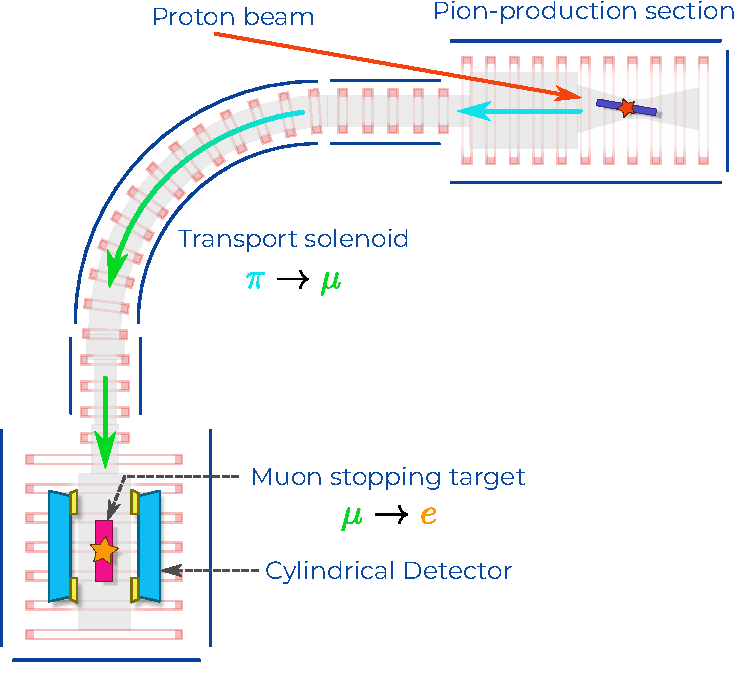
\includegraphics[width=\textwidth]{chapter2/comet_schematic_phase-I.pdf}
        \vspace{3cm}
        \caption{Phase-I with the Cylindrical Detector.}
    \end{subfigure}
    \hfill
    \begin{subfigure}[b]{0.49\textwidth}
        \centering
        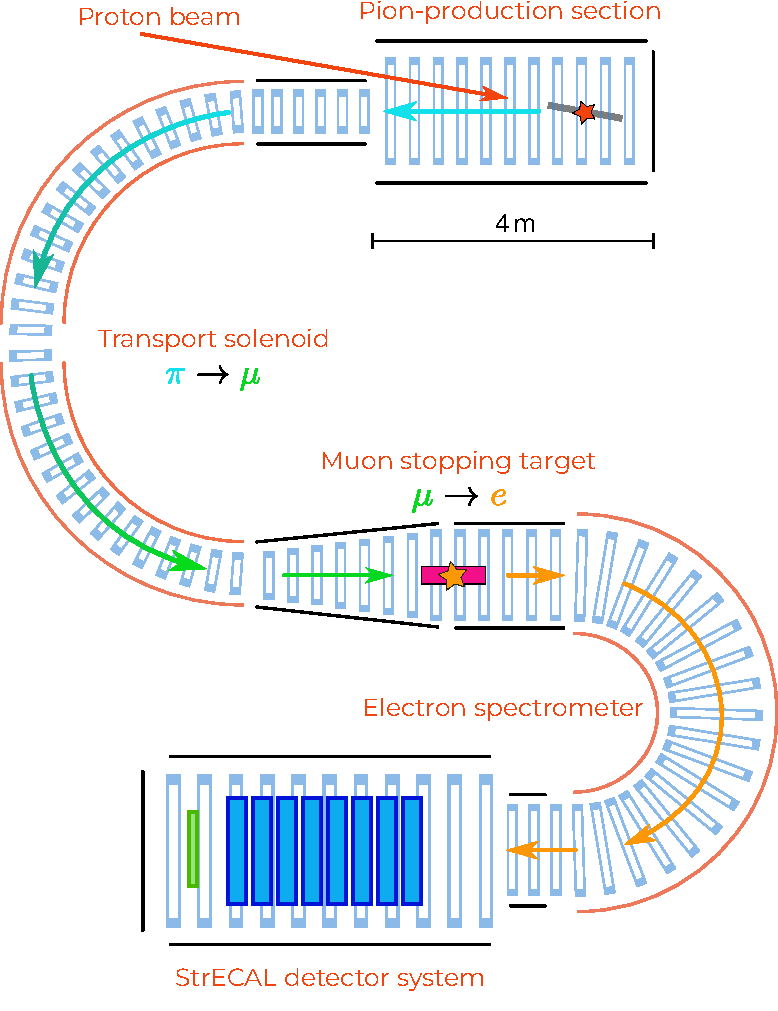
\includegraphics[width=\textwidth]{chapter2/comet_schematic.pdf}
        \caption{Phase-II.}
    \end{subfigure}
    \caption{ Schematic top-down view of the COMET experiment. The light red
        rectangles along the beamline represent solenoids which guide the beam.
        Curved solenoids additionally help to select charge and momentum, as
        discussed in Section~\ref{sec:curved_solenoids}.}
    \label{fig:comet_schematic}
\end{figure}

% \footnote{For $\mu$--$e$ conversion searches, the single-event
% sensitivity (SES) is defined in terms of the fraction of muons captured by the
% target as $\mathrm{SES}(\mu^- N \rightarrow e^- N) = \frac{1}{N_\mu
% f_\mathrm{cap} f_\mathrm{gnd} A_{\mu\mathrm{--}e}}$}

\section{Proton beam}\label{sec:COMET_beam}
Muons in the COMET experiment are produced from the decay of pions produced by
proton collisions on a static solid target. The primary proton beam is provided
by the J-PARC facility. Protons are delivered with an energy of \SI{8}{\GeV},
picked to maximise the pion yield while minimising the production of
anti-protons, a potential background source.

The beam has a pulsed time profile: protons are grouped into \SI{100}{\ns}
bunches, each containing $16\times 10^6$ protons. Bunches are separated by
\SI{1170}{\ns}, which allows conversion signals to be searched for between two
collisions, when the detector is relatively quiet. 

The mean lifetime of a muon bound to an aluminium nucleus is
\SI{864}{\ns}~\cite{PhysRevC.35.2212}, while the \emph{beam flash}, i.e.\ hits
caused by prompt processes just after the proton beam collision, dies off
rapidly within a few hundreds of nanoseconds. Hence, the trigger timing window
can be tuned to reject hits from the beam flash while preserving the acceptance
of electrons from the conversion of bound muons.

% Could also add info on buckets, 4/5 time structure

Stray protons arriving in the time between two bunches can contribute to the
experimental backgrounds by sending particles toward the detector region at
unexpected times. COMET requires the J-PARC proton beam to have fewer than one
such stray proton for every 600 bunches in order to reach its sensitivity goals.
This corresponds to an extinction factor
$$
R_\mathrm{extinction} \equiv \frac{\mathrm{protons\ between\
bunches}}{\mathrm{protons\ per\ bunch}} \approx 10^{-10}.
$$

\section{Pion-production section}

\begin{figure}
    \centering
    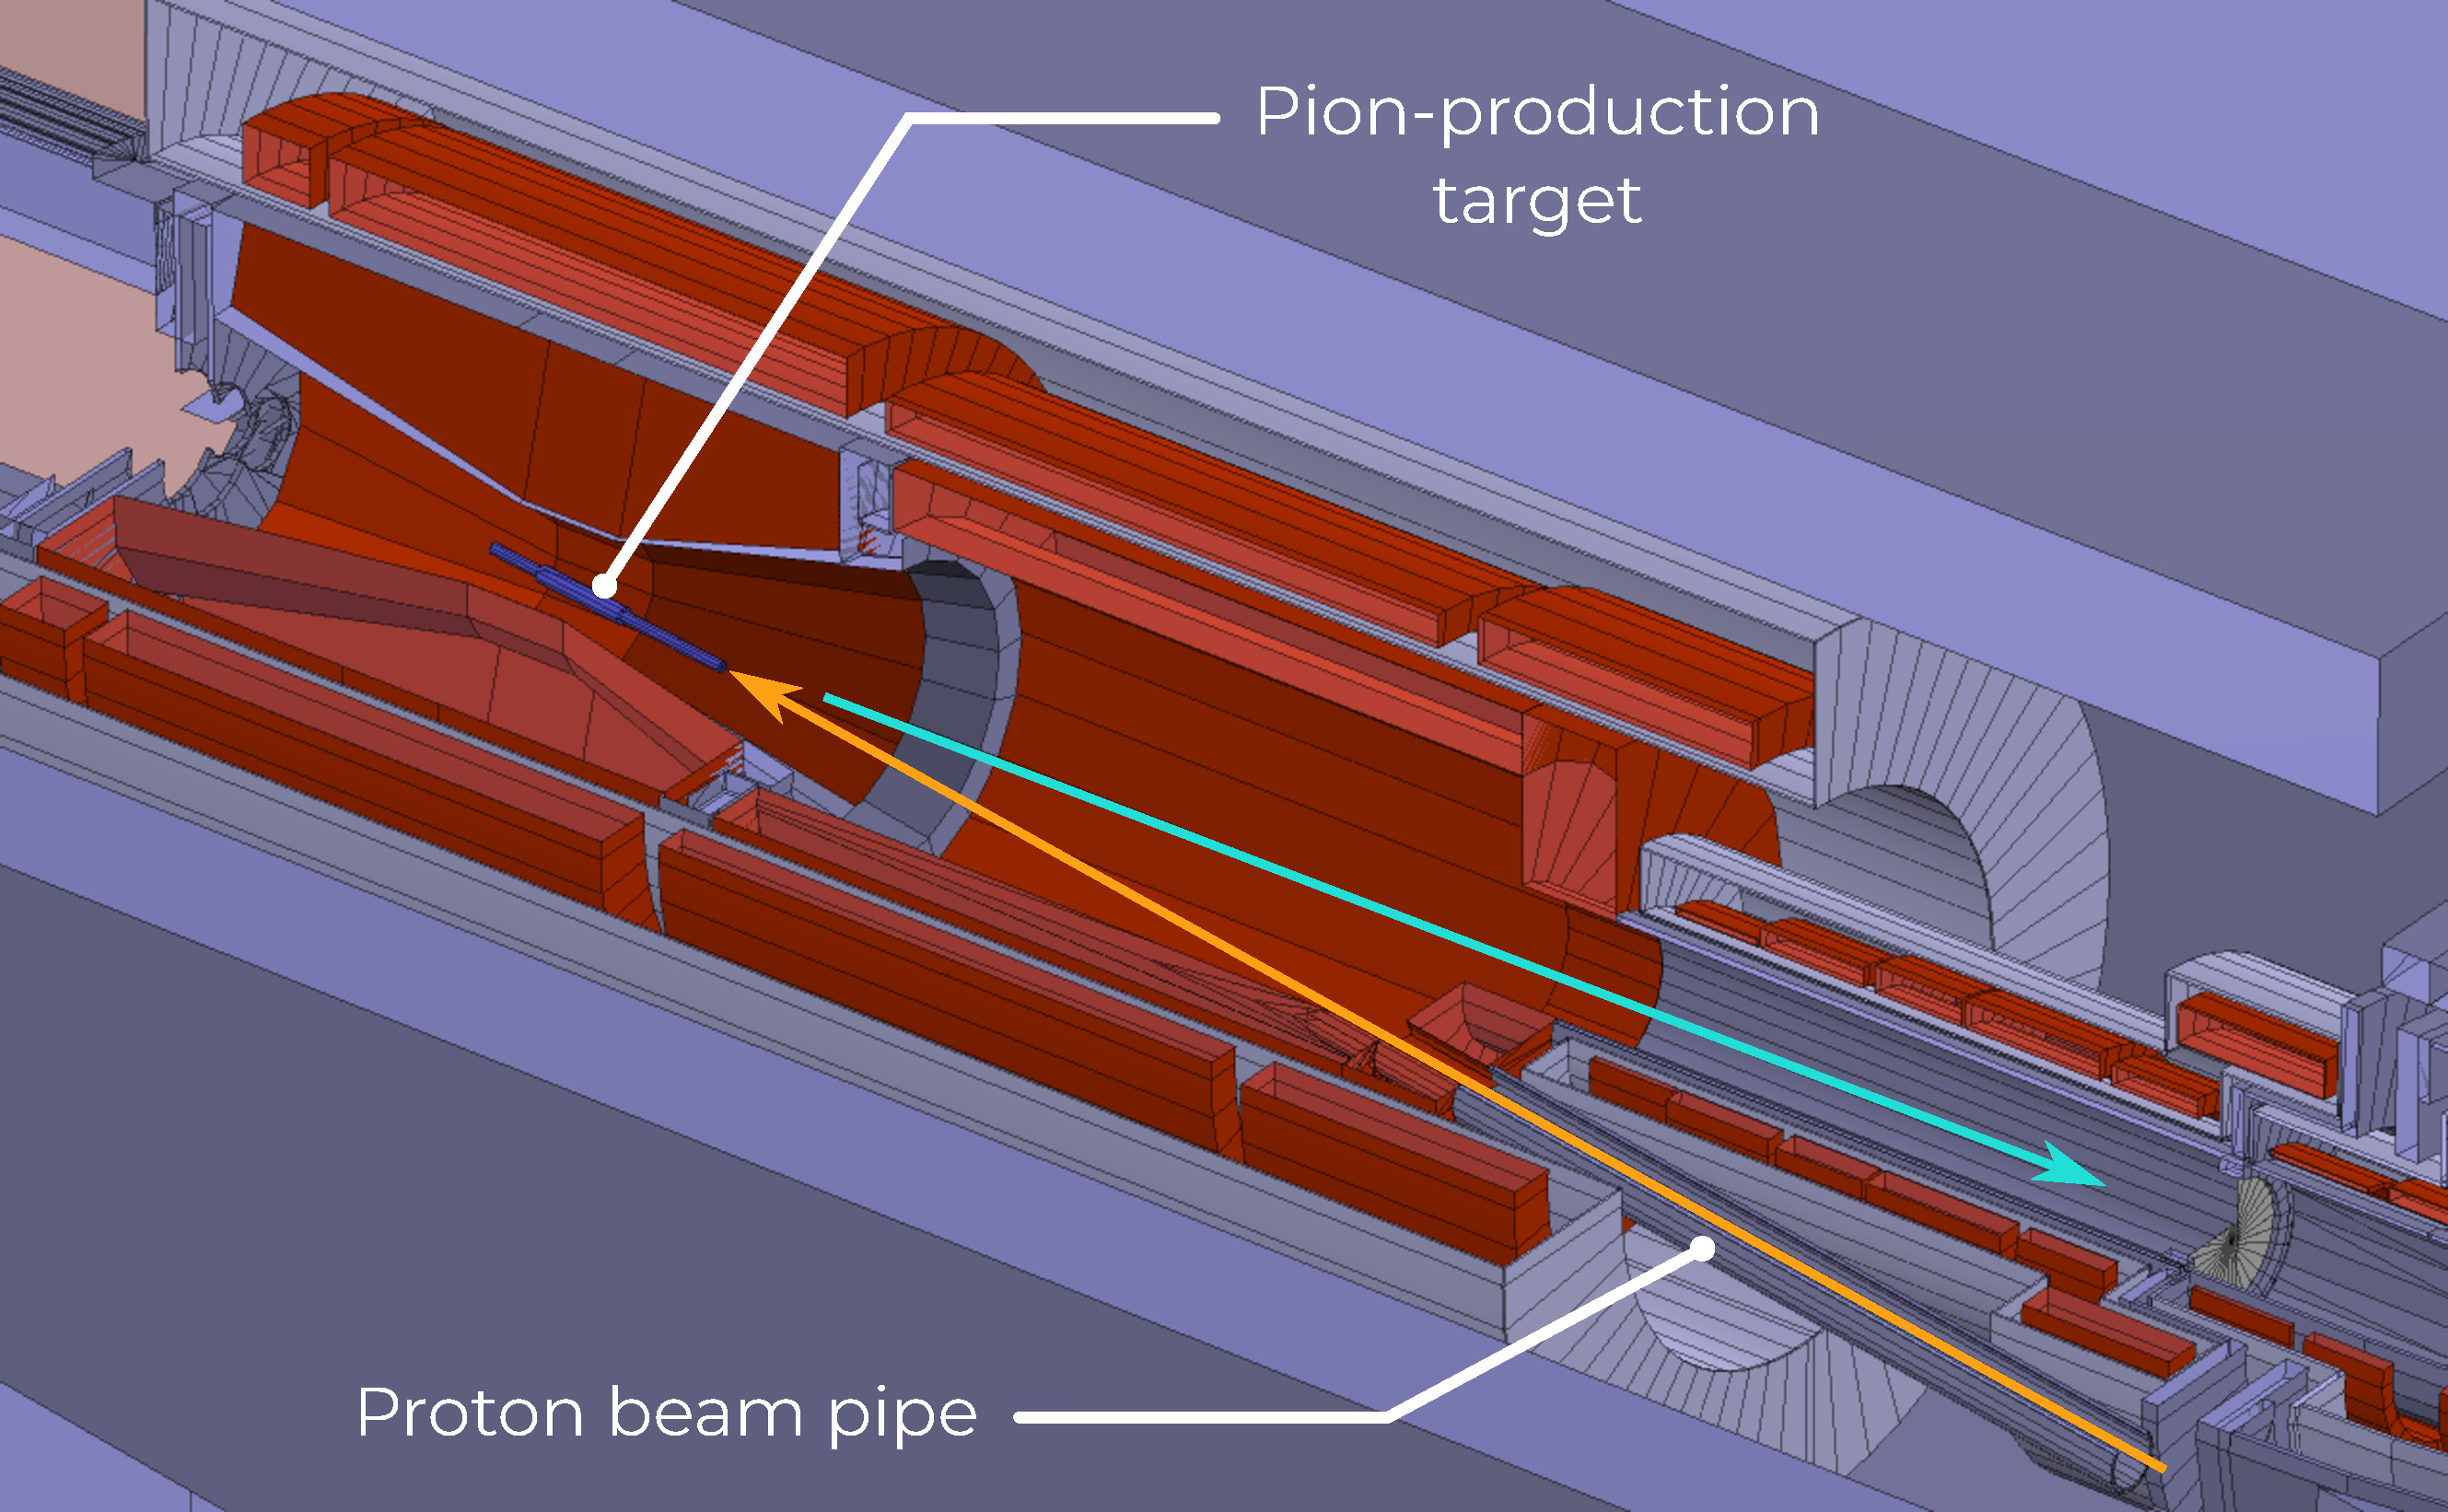
\includegraphics[width=0.8\textwidth]{chapter2/pion_production_section.png.pdf}
    \caption{ Cutaway view of the pion-production section. The orange arrow
        indicates the path of the proton beam while the teal arrow shows the
        direction of backward-going pions captured by the magnetic field.}
    \label{fig:pion_production_section}
\end{figure}

Pions are produced by the collision of the proton beam on a solid target made of
graphite in Phase-I, and tungsten in Phase-II. This region is permeated by a
\SI{5}{\tesla} magnetic field produced by a superconducting solenoid, which
confines the pions and directs them toward the transport solenoid.
Figure~\ref{fig:pion_production_section} shows a cutaway view of this
region.


Pions produced moving backward with respect to the proton beam have a lower
energy than those produced going forward, although they are not as numerous. In
COMET, it is crucial to eliminate high-energy particles in the muon beam that
could produce secondaries mimicking the conversion signal. Hence, the beamline
is positioned in the opposite direction to the proton beam such that only those
low-energy backward-moving pions are allowed into the COMET beamline.
Figure~\ref{fig:pion_momentum} illustrates this by showing that pions moving
backward with respect to the proton beam have a much lower momentum cut-off than
forward-moving pions.

\begin{figure}
    \centering
    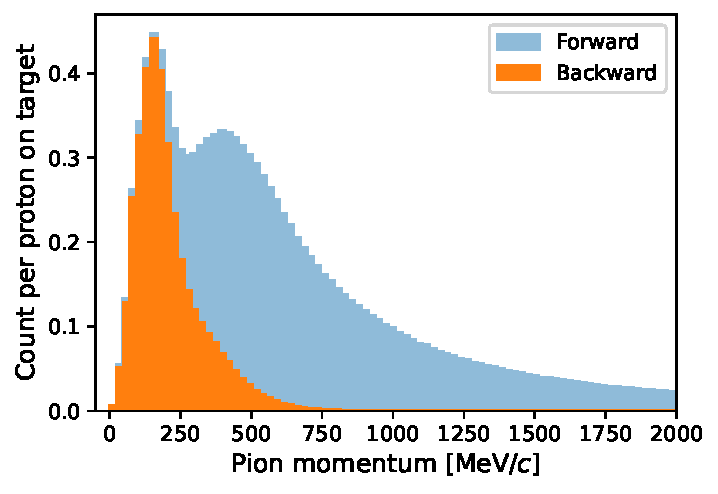
\includegraphics[width=0.5\textwidth]{chapter2/pion_mom-v2.pdf}
    \caption{ Momentum distribution of pions produced by simulating proton
    collisions with Geant4, depending on whether their initial direction is
    forward or backward with respect to the proton beam direction. }
    \label{fig:pion_momentum}
\end{figure}

\section{Transport solenoid}\label{sec:curved_solenoids}

\begin{figure}
    \centering
    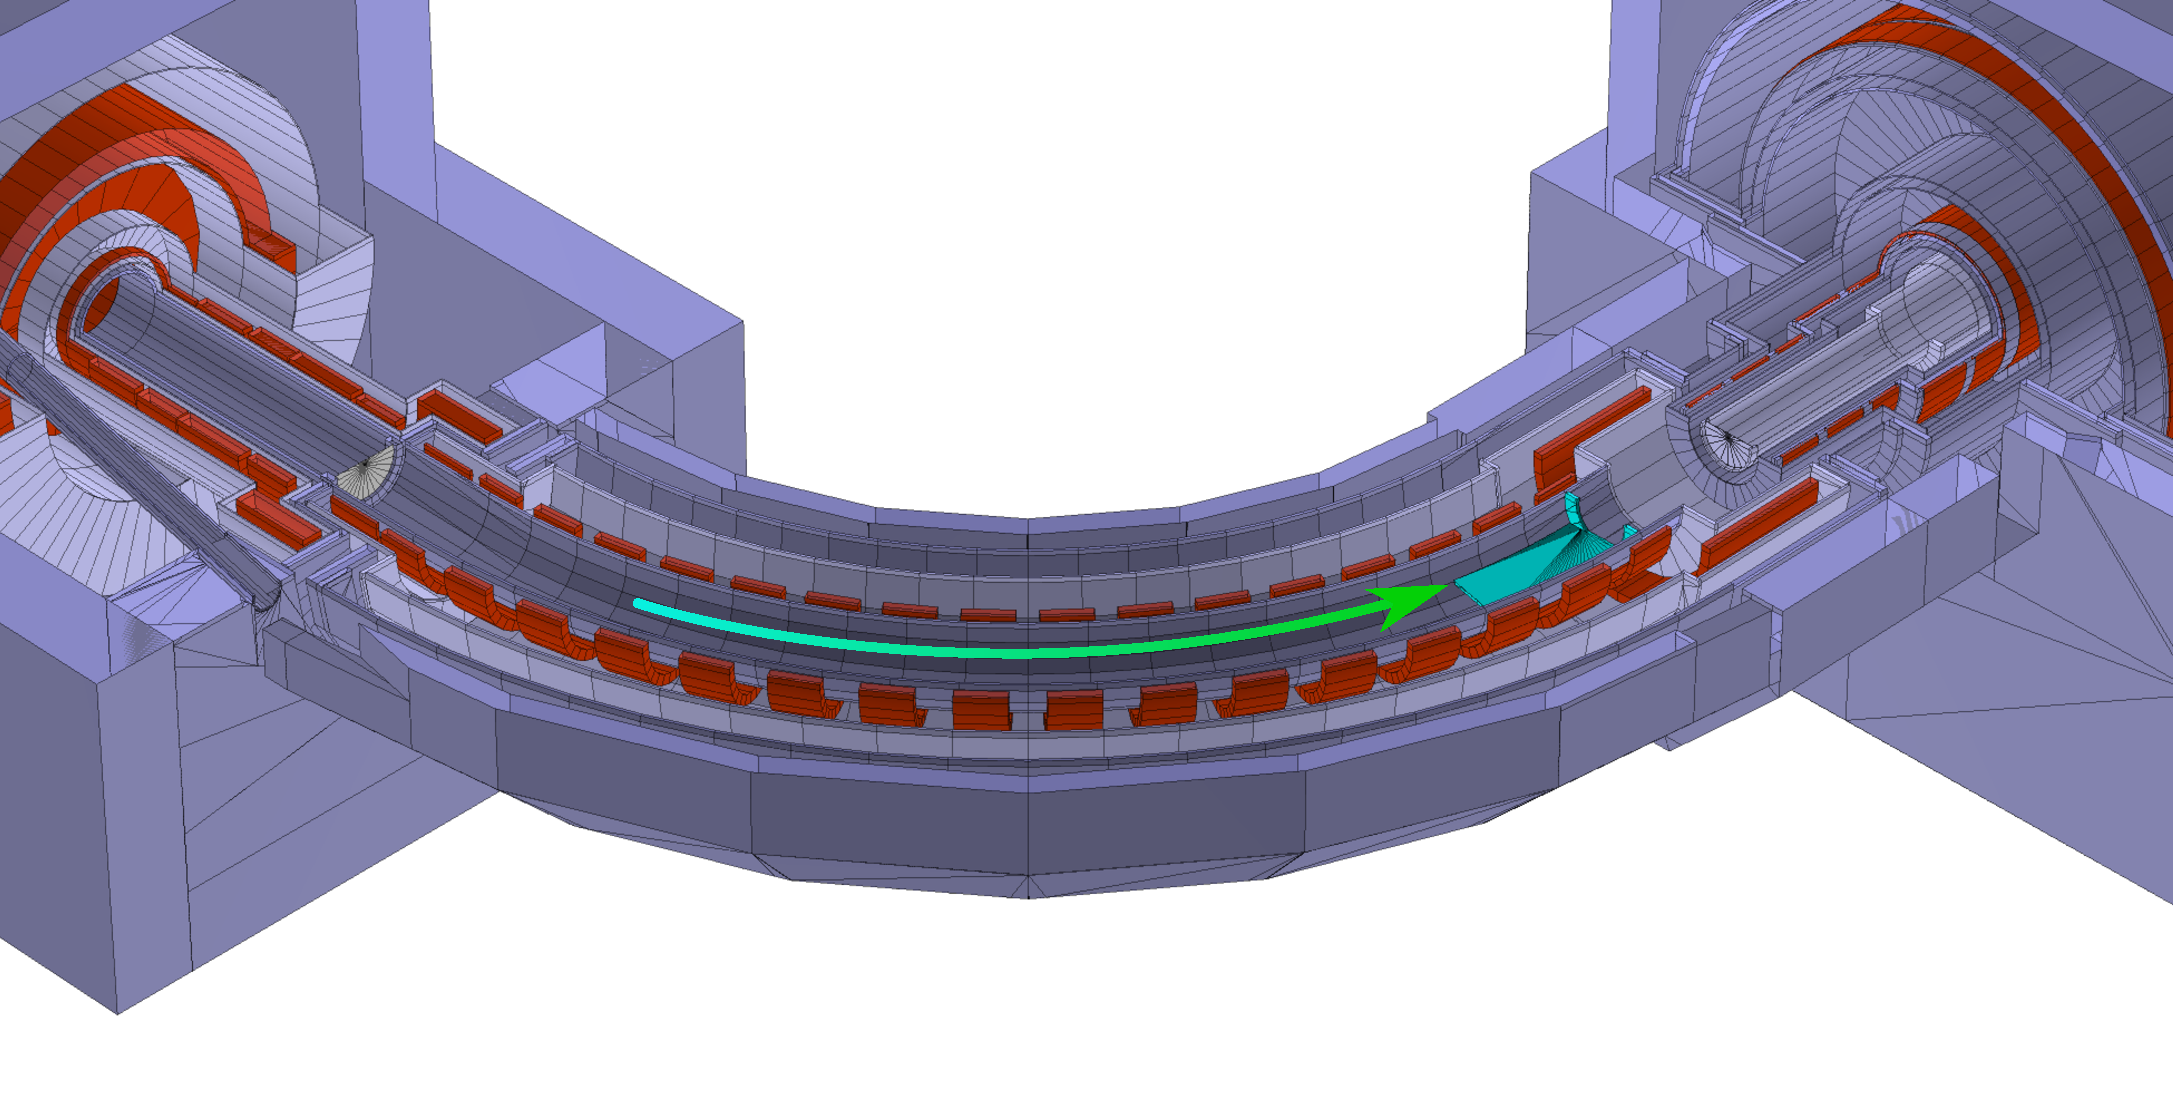
\includegraphics[width=0.8\textwidth]{chapter2/transport_solenoid.pdf}
    \caption{ Cutaway view of the Phase-I transport solenoid. The curved
        solenoid (in red) combined with collimators (in teal) select particles
        depending on their charge and momentum. }
    \label{fig:transport_solenoid}
\end{figure}

The transport solenoid is a curved pipe connecting the pion-production section
to the muon stopping section. Its purpose is twofold: it allows a larger
fraction of pions to decay along the length of the beamline, and the curved
shape combined with its magnetic field and collimators select negatively charged
particles of a specific momentum. 


The magnetic field of a curved solenoid is slightly stronger on the inside of
the curve than on the outside. Since charged particles follow helical
trajectories, this has the net effect of making them drift vertically and the
amount of drift $D$ depends on momentum $p$ according to the equation
\begin{equation*}
    D = \frac{1}{q B} \frac{s}{R} \frac{2 p^2_L + p^2_T}{2 p_L},
\end{equation*}
where $q$ is the charge, $B$ is the strength of the field along the gyration
axis, $s$ is the distance travelled along the solenoid, $R$ is the radius of the
curve, and $p_L$ and $p_T$ respectively denote momentum longitudinal and
transverse to the solenoid axis. From this expression, one can see that
oppositely charged particles drift in opposite directions, and that drift is
overall stronger for higher-momentum particles. The ratio $\frac{p_T}{p_L}$,
which defines a helical trajectory's \emph{pitch angle}, is also a major
factor in a particle's drift.

\begin{figure}
    \centering
    \begin{subfigure}[b]{0.46\textwidth}
        \centering
        \hspace{-0.8cm}
        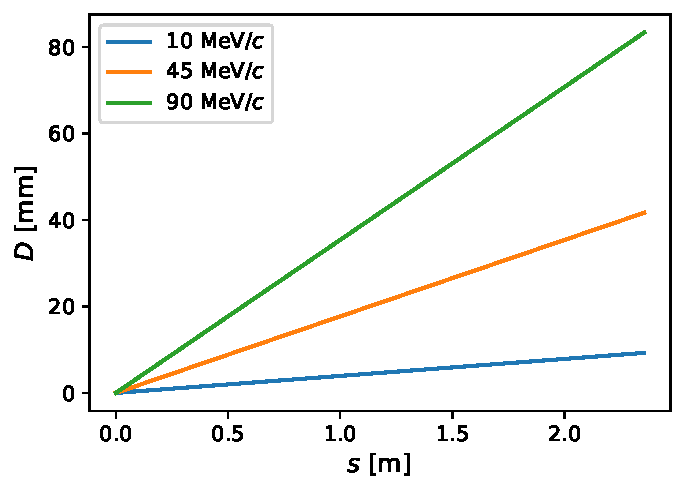
\includegraphics[width=\textwidth]{chapter2/drift_vs_s_0mT.pdf}
        \caption{No dipole field.}
    \end{subfigure}
    \hfill
    \begin{subfigure}[b]{0.46\textwidth}
        \centering
        \hspace{-0.8cm}
        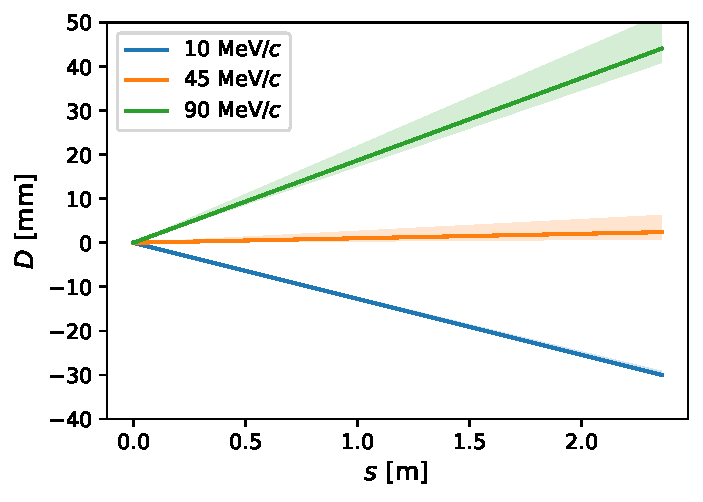
\includegraphics[width=\textwidth]{chapter2/drift_vs_s_0.05mT.pdf}
        \caption{\SI{0.05}{\milli\tesla} vertical dipole field.}
    \end{subfigure}
    \caption{ Effective drift of particles of various momenta as they progress
        along the Phase-I transport solenoid. By applying an additional vertical
        magnetic field, particles of a specific momentum can be selected. Here,
        a \SI{0.05}{\milli\tesla} dipole field allows particles around
        \SI{45}{\MeV/\clight} to stay on axis while higher- and lower-momentum
        particles drift in opposite directions, and can then be suppressed by
        collimators at the end of the transport section. }
    \label{fig:drift}
\end{figure}

The drift caused by the curved solenoid makes all particles of the same charge
move in the same direction to varying degrees depending on momentum. In order to
select particles of a specific momentum, a vertical component is added to the
magnetic field to counterbalance the drift. Selected particles thus stay on
axis, while higher- and lower-momentum particles drift off axis. With the addition
of a collimator at the end of the transport solenoid, particles with unwanted
momenta are effectively eliminated from the beam.

Figure~\ref{fig:drift} shows drift $D$ as a function of $s$, the longitudinal
distance travelled by particles along the solenoid. $D$ is shown for different
values of momentum and assuming the same pitch angle of \SI{45}{\degree}. This
illustrates how, by adding a dipole field, particles with a momentum outside the
required range can be efficiently eliminated by collimators at the top and
bottom of the beam pipe.

\section{Muon stopping target}
The purpose of the muon stopping target is to slow down and stop as many muons
as possible while not blocking the path of conversion electrons. It is composed
of a series of thin aluminium disks placed in the path of the muon beam. The
disks are \SI{20}{\cm} in diameter, \SI{0.2}{\mm} thick, and separated by
\SI{5}{\cm}. The stopping target is shown in Figure~\ref{fig:cydet}, surrounded
by the Cylindrical Detector.

The more aluminium there is, the more muons will be stopped and allowed to
undergo conversion. However, more material means more energy lost by electrons
flying outward, hence the design of the target optimises between muon stopping
rate and acceptance of conversion electrons by the detector system.


The material of the stopping target influences the conversion rate, but also the
lifetime of a muon caught in orbit around a nucleus. A heavy target favours the
expected rate of $\mu$--$e$ conversion, however it also causes the nuclear
capture rate to be higher. In COMET, beam bunches are separated by
\SI{1.17}{\ns} and prompt backgrounds typically die off within a few hundred
nanoseconds. A muonic atom with an iron or heavier nucleus has a lifetime less
than \SI{200}{\ns}, which would be too short to allow muons to stay bound and
convert after the beam flash is over. Hence, a light target such as aluminium,
with a longer stopped muon lifetime of \SI{864}{\ns}, is better suited to the
COMET conversion search.

\section{Detector systems}
\subsection{StrECAL}
The StrECAL combines a straw-tube tracking detector with an electromagnetic
calorimeter for energy measurement. In COMET Phase-I, the StrECAL will serve as
a beam characterisation apparatus. It will be placed directly at the end of the
transport solenoid, without a muon stopping target, to study the composition of
the COMET beam and gain a more thorough understanding of potential backgrounds.
The collected data can also serve to validate and refine the Monte Carlo
simulation in preparation for the conversion measurement.

In COMET Phase-II, the StrECAL will serve as the detector system for the
conversion measurement. It will be placed after the electron spectrometer, a
curved solenoid section tuned to select conversion electrons, as shown in
Figure~\ref{fig:comet_schematic}. Figure~\ref{fig:strecal} shows a rendering of
the StrECAL detector system in Phase-II.

The Straw Tracker uses thin straw tubes as drift chambers, arranged into
circular planes. A series of stations, each one able to measure the horizontal
and vertical position of a particle, are positioned along the beam direction. A
spatial resolution of less than \SI{100}{\um} allows the Straw Tracker to
reconstruct trajectories and estimate particle momenta via time-of-flight
information.

The ECAL is a crystal electromagnetic calorimeter which supplements the Straw
Tracker in measuring energy and thus identifying electrons. The ECAL uses
lutetium-yttrium oxyorthosilicate (LYSO) as its scintillating crystals and
avalanche photodiodes to collect the emitted photons.


\begin{figure}
    \centering
    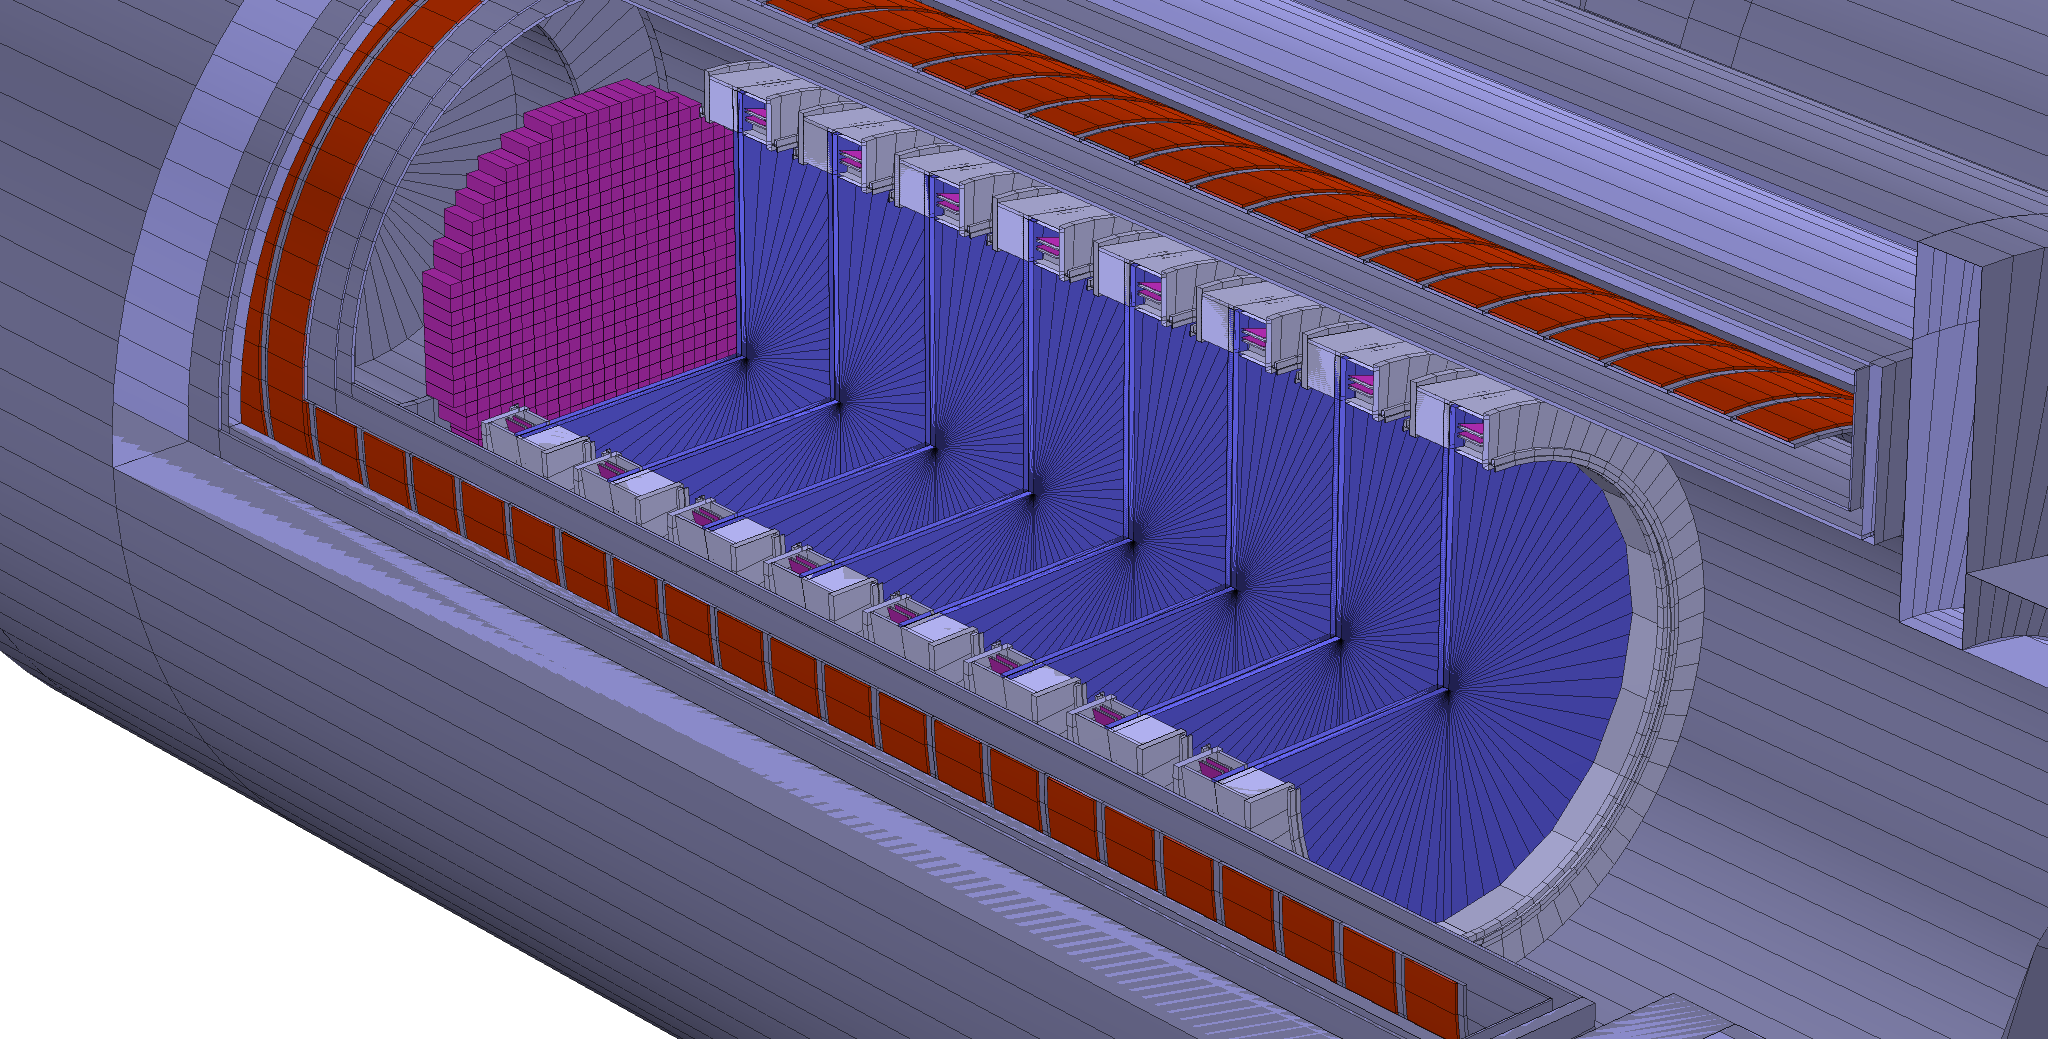
\includegraphics[width=0.8\textwidth]{chapter2/strecal.png}
    \caption{ Cutaway view of the StrECAL detector. The ECAL is shown in
        purple and the Straw Tracker stations in blue. }
    \label{fig:strecal}
\end{figure}

\subsection{CyDet}
The Cylindrical Detector (CyDet) consists of a Cylindrical Drift Chamber (CDC)
for tracking and a Cylindrical Trigger Hodoscope (CTH) for triggering on
specific event signatures. The CyDet surrounds the muon stopping target and sits
within the detector solenoid which generates a \SI{1}{\tesla} longitudinal
magnetic field. This configuration is designed to eliminate backgrounds from the
beam itself as well as low-momentum products of the collision while maximising
the acceptance of conversion electrons.
Figure~\ref{fig:cydet} shows a rendering of the Cylindrical Detector.

\begin{figure}
    \centering
    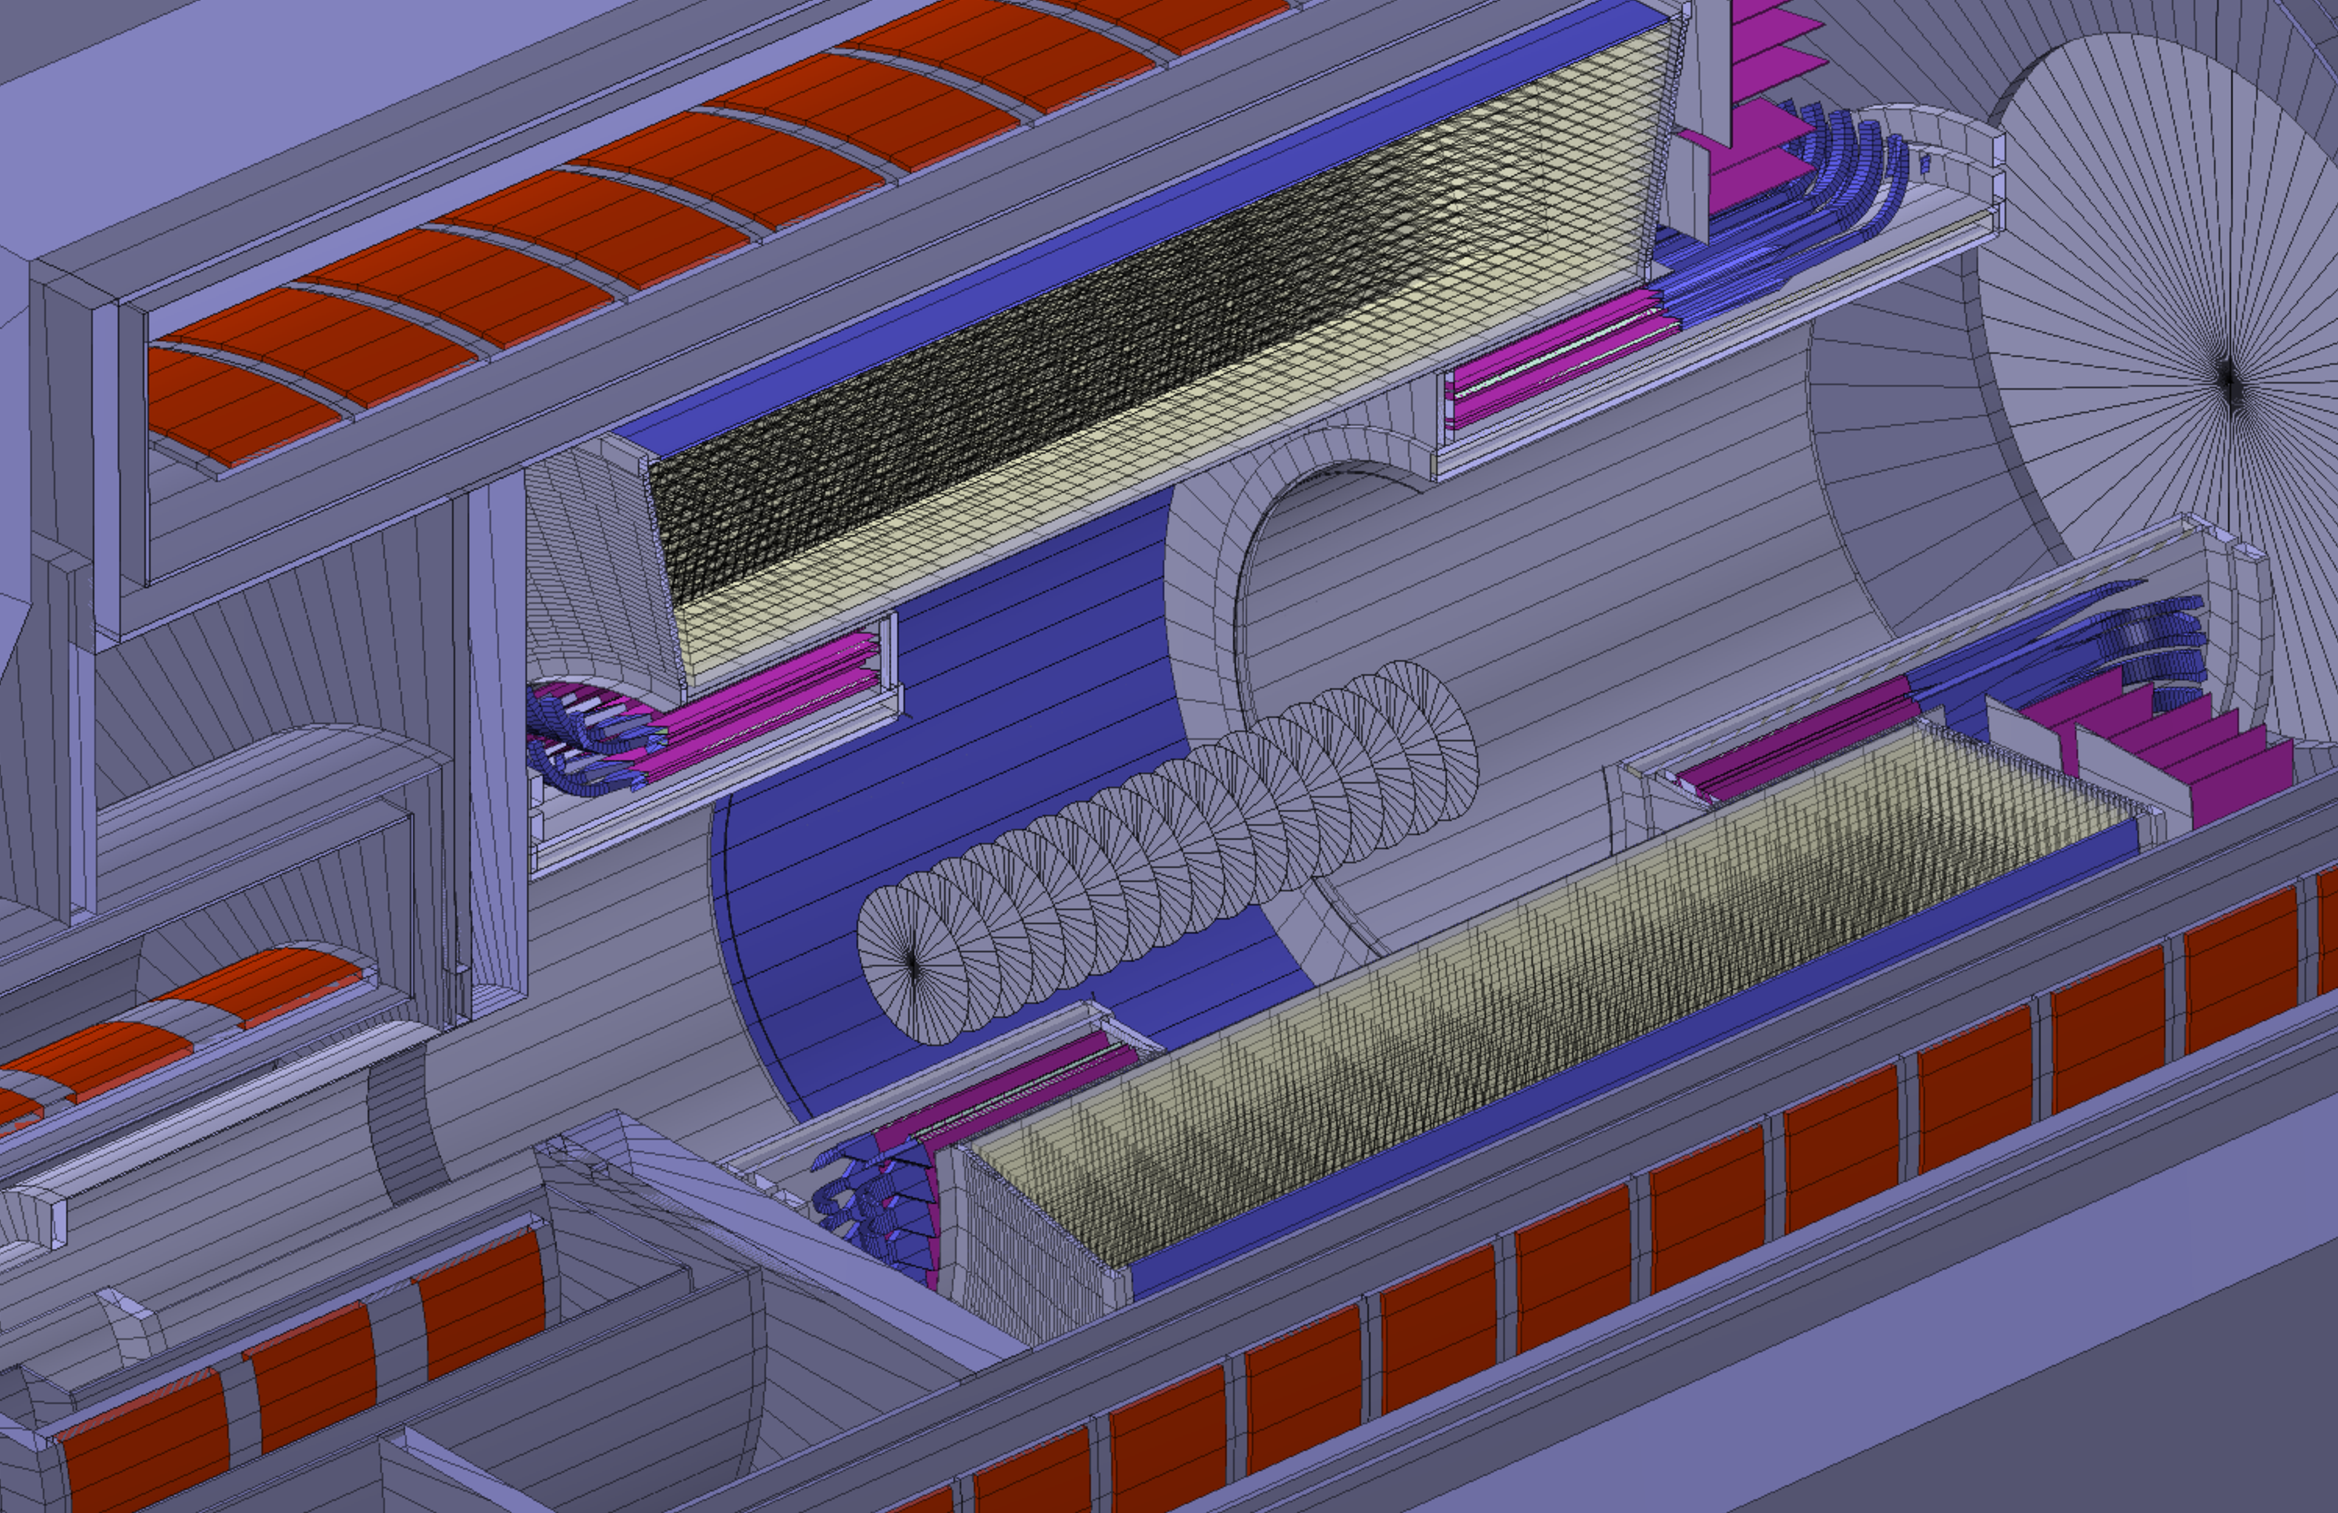
\includegraphics[width=0.8\textwidth]{chapter2/cydet.pdf}
    \caption{ Cutaway view of the Cylindrical Detector, composed of the
        Cylindrical Drift Chamber (in beige) and Cylindrical Trigger Hodoscope
        (in purple). The detector solenoid coils are visible in red, and the
        muon stopping target disks sit in the centre of the detector system.
        \hl{TODO change color of RECBEs so they're different from CTH counters.}
        }
    \label{fig:cydet}
\end{figure}

The CDC is a drift chamber used to track charged particles emanating from the
muon stopping target. It has an inner radius of \SI{50}{\cm}, which prevents
charged particles produced in the muon beam collision whose transverse momentum
is smaller than \SI{60}{\MeV/\clight} from reaching it. 

The CDC has 4986 sense wires strung out longitudinally in 20 concentric layers.
Layers have an alternating stereo angle, whereby the wires in a layer are
rotated slightly either clockwise or anti-clockwise with respect to the axis.
This special property allows the drift chamber to roughly resolve the
longitudinal position of a particle in addition to its radial and azimuthal
position. The ionising material in the CDC is a helium-isobutane mixture.

% CDC efficiency: geometric acceptance?

\subsection{Cosmic ray veto}
The COMET experiment hall is constantly irradiated by muons produced in the
atmosphere by cosmic rays. The cosmic ray veto (CRV) is an additional active detector
which surrounds the CyDet or StrECAL detector system. Its purpose is to identify
events induced by cosmic muons rather than by the COMET beam, and thus reduce
the probability that such events will be mistaken for the conversion signal.

% Do we need to describe the CRV? Can we just say it needs to have X efficiency.
The CRV is composed of four layers of scintillator. \hl{Not all of it. GRPC.}

\section{Conversion signature}
Conversion electrons are mono-energetic and emitted isotropically by muons
stopped in the target disks. In the magnetic field of the detector solenoid,
they have a helical trajectory which can be reconstructed by the CDC or Straw
Tracker.

% Timing

% Trigger criteria


\section{Experimental backgrounds}\label{sec:backgrounds}
The COMET experiment is specifically designed to be sensitive to a $\mu$--$e$
conversion signal, i.e.\ to eliminate as many sources of background as possible
while making sure to notice the process if it does occur. 

Observing $\mu$--$e$ conversion requires the production of an intense source of
muons which must be bound to atomic nuclei. COMET uses a proton beam from the
J-PARC main ring.


The COMET experiment will produce a muon beam and direct it toward a static
aluminium target to slow down and stop the muons. As discussed in
Section~\ref{sec:sm_backgrounds}, a bound muon can undergo decay in orbit (DIO)
or nuclear capture.

% Antiprotons

\section{Sensitivity}\label{sec:SES}



% The choice of target material directly influences how frequently high-energy
% electrons will be produced by these processes, and hence contributes in
% setting the maximum experimental sensitivity.

% This should go into the COMET section as these are specific to COMET and/or
% specifically addressed by the COMET design.
% Background events can be classified into three categories: intrinsic,
% beam-related, and cosmic ray-induced.

% Beam-related backgrounds come from impurities in the high-intensity muon beam.
% The specifics of the COMET beam and how these backgrounds are alleviated is
% discussed in Section~\ref{sec:COMET_beam}.

% Cosmic rays typically produce muons with a wide range of energies in the
% atmosphere which 